\section{Método del trapecio}

	\subsection{Introducción}

		\begin{frame}{Introducción al método del trapecio}
			\fontsize{11}{11}\selectfont				
			\begin{proposition} \label{prop:sol-eq}
				Sea un PVI con $y'(t) = f(t,y(t))$ y $y(t_0) = y_0$.  Son equivalentes:
				\begin{enumerate}
					\item $y$ es una solución del PVI.
					\item $y(t) = y_0 + \int_{t_0}^{t} f(s,y(s))) ds \ \forall t \in [a,b]$
				\end{enumerate}
			\end{proposition}

			\kern 7mm
			\begin{tcolorbox}[colback=ChetwodeBlue!10,colframe=ChetwodeBlue!60]
				Nuestra solución verifica:
				\begin{equation*}
					y(t_1)  = y_0 + \int_{t_0}^{t_1} f(s,y(s))) \ ds
				\end{equation*}		
			\end{tcolorbox}
		\end{frame}

		\begin{frame}{Introducción al método del trapecio}
			\fontsize{10}{10}\selectfont				

			\begin{tcolorbox}[colback=ChetwodeBlue!10,colframe=ChetwodeBlue!60]
				\centering
				\textbf{Idea: Método del trapecio para integración numérica}
				\begin{equation} \label{eq:trapecio-igualdad}
					y(t_{1}) = y_0 + \frac{h}{2} \left[f(t_0,y_0) + f(t_1, y(t_1))\right] - \frac{h^3}{12}y^{3)}(\xi)
				\end{equation}

				\textbf{Aproximación implicita}	
				\begin{equation} \label{eq:app}
					y(t_1) \approx w_1 = w_0 + \frac{h}{2} \left[f(t_0,w_0) + f(t_1, y(t_1))\right]
				\end{equation}			
			\end{tcolorbox}			

			\kern 1mm
			\centering
			\textbf{¿Cómo cálcular la aproximación?}

			\kern 1mm
			\begin{itemize}
				\item \color{ChetwodeBlue}\textbf{Método del trapecio explícito}
				\item \color{ChetwodeBlue}\textbf{Método del trapecio implícito}
			\end{itemize}
		\end{frame}

	\subsection{Método del trapecio explícito}


		\begin{frame}{Método del trapecio explícito}
			\fontsize{10}{10}\selectfont		
			\centering
			\begin{tcolorbox}[colback=ChetwodeBlue!10,colframe=ChetwodeBlue!60]
				\centering
				\textbf{Idea: Utilizar el método de Euler}
				\begin{equation*}
					y(t_{i+1}) \approx w'_{i+1} = w'_i + h f(t_i,w'_i))
				\end{equation*}
				{\large\textbf{+}}
				\begin{equation*}
					y(t_{i+1}) \approx w_{i+1} = w_i + \frac{h}{2} \left[f(t_i,w_i) + f(t_{i+1}, y(t_{i+1}))\right]
				\end{equation*}			
			\end{tcolorbox}			

			 \begin{definition}[Método del trapecio explícito]
				\begin{equation} \label{eq:app-exp}
					y(t_{i+1}) \approx w_{i+1} = w_i + \frac{h}{2} \left[f(t_i,w_i) + f(t_{i}+h, w_i + h f(t_i,w_i))\right]
				\end{equation}
			 \end{definition}
			
		\end{frame}

		\begin{frame}{Comparación con el método de Euler}
			\fontsize{10}{10}\selectfont		
			\centering
			\kern3mm
			Denotamos
			\begin{cases}
				$S_L = h f(t_i,w_i)$ \\
				$S_R = h f(t_{i+1}, w_i + S_L)$ \\
			\end{cases}

			\kern3mm
			\begin{itemize}
				\item \textbf{Método de euler:} $w'_{i+1} = w_i + S_L$
				\item \textbf{Método del trapecio explícito:} $w_{i+1} = w_i + \frac{S_L + S_R}{2}$
			\end{itemize}

			\kern3mm
			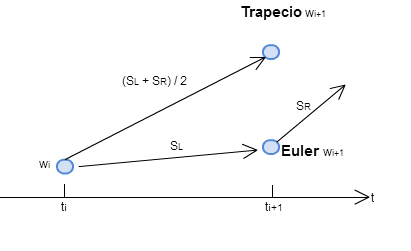
\includegraphics[width=0.65\textwidth]{./Images/trapecio-vs-euler.png}
		\end{frame}
		
		\begin{frame}{Error local y global}
			\begin{theorem}
				El método del trapecio es localmente de orden tres. \\
				En consecuencia, el método del trapecio es de orden dos.
			\end{theorem}
			
			\begin{proof}
				Se basa en el teorema de Taylor.
			\end{proof}

			\begin{corollary}
				El método del trapecio explícito es convergente.
			\end{corollary}
		\end{frame}
		
		\begin{frame}{Error de redondeo}
			\centering
			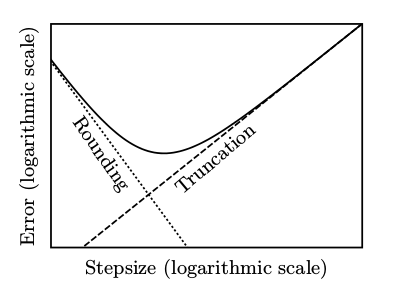
\includegraphics[width=0.65\textwidth]{./Images/redondeo.png}
		\end{frame}
		
		\begin{frame}{Estabilidad y convergencia}
			\textbf{Función de incremento:} $\phi(t,y,h)=\frac{1}{2}f(t,y)+\frac{1}{2}f(t+h,y+hf(t,y))$
			
			\begin{proposition}
				Si $f: \Omega \rightarrow \mathbb{R}$ es lipschitziana respecto de la segunda variable, entonces $\phi$ es lipschitziana respecto de la segunda variable en $\Omega \times [0, h_0]$ para cualquier $h_0$.
			\end{proposition}
			
			\begin{corollary}
				El método del trapecio explícito es estable y consistente.
			\end{corollary}
			\begin{proof}
				Teorema de consistencia, convergencia y estabilidad.
			\end{proof}
		\end{frame}